\label{section:problema}

\todo{CS4002}
\todo[color=blue!40]{CS4003}
\todo[color=green!40]{CS4004}

Los fragmentos de fósiles, huesos fracturados y objetos de herencia cultural, por lo general, requieren ser ensamblados para su futuro estudio. En específico, podemos dividir el problema en dos etapas: la correspondencia y la alineación. La primera etapa consiste en extraer características de las caras fracturadas de los fragmentos para encontrar cuáles deben unirse. La segunda etapa consiste en encontrar la transformación por la cual deben pasar los fragmentos para minimizar la distancia y evitar la superposición. En la figura \ref{fig:brick} se observa el proceso de reensamblaje en el modelo \textit{brick} del \textit{dataset} GMIG \cite{13}.

\begin{figure}[!h]
    \centering
     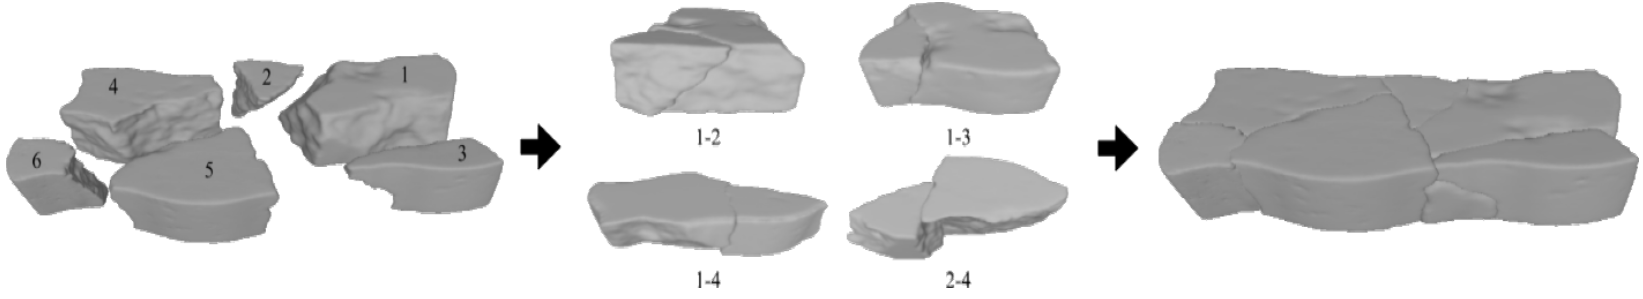
\includegraphics[scale=0.21]{images/brick.png}
    \caption{Reconstrucción del modelo \textit{Brick} (GMIG)}
    \label{fig:brick}
\end{figure}

\newpage

Por otro lado, hasta donde tenemos conocimiento, los métodos actuales no han profundizado en el uso de técnicas de \textit{deep learning} para las etapas de correspondencia y alineación. En tal sentido, esta tesis presenta un nuevo método basado en técnicas de \textit{deep learning} para resolver el problema de reensamblaje de objetos 3D rígidos con fragmentos gruesos no erosionados.
